\documentclass[conference]{IEEEtran}
\IEEEoverridecommandlockouts
\usepackage{cite}
\usepackage{amsmath,amssymb,amsfonts}
\usepackage{algorithmic}
\usepackage{graphicx}
\usepackage{textcomp}
\usepackage{xcolor}
\usepackage{algorithm}
\usepackage{booktabs}
\usepackage{multirow}
\usepackage{array}
\usepackage{balance}
\def\BibTeX{{\rm B\kern-.05em{\sc i\kern-.025em b}\kern-.08em
    T\kern-.1667em\lower.7ex\hbox{E}\kern-.125emX}}
\begin{document}

\title{SHAP-$\sigma$: A Label-Free Rashomon Pipeline\\for Multivariate Time-Series Anomaly Detection\\
\thanks{The \textit{Rashomon-based Uncertainty-Aware Explainable AI for Time Series} has received funding from the European Union, via the OC4-2025-TES-02 issued and implemented by the ENFIELD project, under the grant agreement No 101120657.}
\thanks{Code and data for full reproducibility: \texttt{https://github.com/ugurdar/shap\_sigma\_paper}.}
}

\author{\IEEEauthorblockN{Ugur Dar$^{1*}$, Sara Malacarne$^{2}$, Mustafa Cavus$^{1}$, Jeriek Van den Abeele$^{2}$}
\IEEEauthorblockA{$^{1}$Eskisehir Technical University, Department of Statistics, Eskisehir, T\"urkiye\\
$^{2}$Telenor Research and Innovation, Oslo, Norway\\
{*ugurdarr@gmail.com}
}}

\maketitle

\begin{abstract}
We address unsupervised anomaly detection on multivariate cellular
network KPI streams, where labels are unavailable for both training
and model selection. Existing label-free quality criteria such as the
Mass--Volume curve~\cite{Goix2016} are known to be noisy, and
single-detector SHAP explanations cannot signal when a flag should be
trusted. We propose \textbf{SHAP-$\sigma$}, a label-free pipeline for
per-KPI multivariate anomaly detection that
(i) self-tunes a pool of $K{=}10$ unsupervised detectors label-free
(PCA via $95\%$ explained variance; $k$-NN/LOF via the $k$-distance
elbow; GMM via BIC; HBOS via Sturges' rule; an AutoEncoder whose
bottleneck width inherits the tuned PCA dimension; OCSVM and IF on
robust defaults; ECOD/COPOD parameter-free);
(ii) selects a small \emph{Rashomon set} of $K_R$ detectors via a
closed-form joint pair score that combines a Mass--Volume proxy with
a cardinality veto (eliminating constant-output detectors);
(iii) explains every selected detector with a LightGBM surrogate and
TreeSHAP; and (iv) uses the cross-detector standard deviation of those
attributions as a per-KPI gate that corroborates anchor flags.
On TELCO ($12$ per-KPI label streams), the pipeline reaches per-KPI
macro $F_1{=}0.464$ at $K_R{=}4$ with precision $0.605$ and recall
$0.425$, against $0.419$ (LOF, the best self-tuned singleton). The
pipeline exceeds the released deep baselines DC-VAE
($F_1{=}0.134$~\cite{gonzalez2023one}) and
C-MTAD-GAT ($F_1{=}0.160$~\cite{Malacarne2026}) by $2.9$--$3.5\times$
on the same evaluation window, while remaining fully transparent
(per-KPI SHAP attributions) and reproducible.
\end{abstract}

\begin{IEEEkeywords}
time series, anomaly detection, SHAP, Rashomon, unsupervised model selection, XAI
\end{IEEEkeywords}

\section{Introduction}
\label{sec:intro}

Unsupervised anomaly detection in multivariate time series underpins
fault diagnosis in domains as diverse as cellular networks, server
fleets, and industrial telemetry. Yet a persistent obstacle hinders
deployment: without ground-truth labels, the practitioner cannot
reliably decide which detector to trust. Internal validation metrics
that work well for clustering rarely transfer to anomaly detection,
and recent large-scale empirical work shows that most label-free
criteria perform near random when ranking modern
detectors~\cite{MaZhao2023}.

This selection problem is sharpened by the \emph{Rashomon
effect}~\cite{Breiman2001}: for any non-trivial task, a multiplicity
of near-optimal models exists, each making different
errors~\cite{Semenova2022,Fisher2019}. We argue that this attribution
disagreement is not noise to be averaged away but a signal to be
exploited: at a flagged point, the spread of attributions across the
Rashomon set indicates that at least one detector commits to a
feature-level explanation, providing second-source evidence beyond
the anchor's score.

Prior label-free model selection has explored three avenues.
Excess-Mass and Mass-Volume curves~\cite{Goix2016} give geometry-based
scores but assume well-behaved density estimates. Meta-learning
approaches such as MetaOD~\cite{Zhao2021} and ELECT~\cite{Zhao2022}
transfer historical-performance signals across datasets, but require
an offline labelled meta-corpus. Most recently, robust Borda rank
aggregation across multiple imperfect internal metrics has been
proposed for time-series AD~\cite{Goswami2023}; the large-scale study
of~\cite{MaZhao2023} shows that no internal metric universally
dominates. PyOD~\cite{Zhao2019} has standardized detector
implementations. None of these methods exploit \emph{feature
attribution} as a selection signal.

Independently, SHAP~\cite{Lundberg2017,Lundberg2020} has become the
de facto post-hoc explainer for anomaly detection, mostly to explain a
single chosen model; the closest precedent is Levy et
al.~\cite{Levy2026}, who use SHAP attributions for ensemble member
\emph{selection} in supervised tabular AD, whereas we use cross-detector
SHAP standard deviation as an attribution-evidence \emph{gate} in the
unsupervised TS regime. Modern deep TS-AD
methods~\cite{Audibert2020,Tuli2022,Xu2022,Yang2023} likewise commit
to a single architecture. Outlier ensemble
theory~\cite{AggarwalSathe2017,Zimek2014}
and the classical diversity literature~\cite{Kuncheva2003} establish
that complementary errors improve ensemble accuracy, yet the standard
diversity measures (Q-statistic, disagreement) require labels.
Following~\cite{Zimek2014}, we replace label-dependent diversity with
the Spearman rank correlation of training scores, which~\cite{Zimek2014}
identifies as the practical label-free proxy in OD ensembles.

\paragraph{Contributions.}
(1) Label-free self-tuning of the entire PyOD detector pool
(PCA via $95\%$ explained variance; $k$-NN/LOF via $k$-distance elbow;
GMM via BIC; HBOS via Sturges' rule), which raises detector-level
$F_1$ without using any anomaly labels.
(2) A closed-form Rashomon pair score
$s_{ij}=\tfrac{1}{2}(q_i+q_j)(1-\rho_{ij})$, where $q_d$ combines a
Mass--Volume proxy with a cardinality veto (eliminating
constant-output detectors), jointly rewarding label-free quality and
inter-detector score decorrelation.
(3) A $\sigma$-SHAP attribution-evidence filter using cross-detector
SHAP standard deviation as a second-source signal that corroborates
anchor flags on per-KPI labels.
(4) Empirical demonstration on the TELCO cellular benchmark
that the closed-form pair score identifies the empirical oracle pair
label-free, and the pipeline exceeds the best singleton and recent
deep baselines DC-VAE and C-MTAD-GAT~\cite{Malacarne2026,gonzalez2023one}.

\paragraph{Literature gap.}
To our knowledge, no published method combines (a) label-free detector
selection with (b) SHAP attributions as a \emph{filter} signal rather
than a post-hoc explanation. Rashomon-set analysis has so far been
developed in supervised regimes~\cite{Semenova2022,Fisher2019}; its
extension to unsupervised anomaly detection is open. Robust rank
aggregation~\cite{Goswami2023} pools imperfect label-free metrics but
never inspects attributions, while~\cite{MaZhao2023} diagnoses their
weakness without proposing a disagreement-based pipeline.
SHAP-$\sigma$ promotes the cross-detector standard deviation of
attributions from an explanatory afterthought to a first-class,
label-free attribution-evidence signal.

The remainder of the paper is organized as follows.
Section~\ref{sec:method} formalizes joint pair scoring and the
$\sigma$-SHAP filter. Section~\ref{sec:exp} describes datasets and
protocol. Section~\ref{sec:results} reports empirical results.
Section~\ref{sec:conclusion} concludes.

\section{Methodology}
\label{sec:method}

We propose \textbf{SHAP-$\sigma$}, a label-free pipeline that selects a
small subset $\mathcal{R}\subseteq\mathcal{D}$ of detectors from a pool
$\mathcal{D}$ by jointly optimising label-free quality and pairwise
diversity, explains every member of $\mathcal{R}$ with a tree
surrogate, takes TreeSHAP attributions~\cite{Lundberg2017,Lundberg2020},
and converts the cross-detector spread of those attributions into a
per-point, per-feature attribution-evidence gate. Labels are used
nowhere in training, ranking, or set selection.

\subsection{Notation}
Let $X_{\mathrm{tr}}\!\in\!\mathbb{R}^{N_{\mathrm{tr}}\times p}$,
$X_{\mathrm{v}}\!\in\!\mathbb{R}^{N_{\mathrm{v}}\times p}$, and
$X_{\mathrm{te}}\!\in\!\mathbb{R}^{N_{\mathrm{te}}\times p}$ denote
the training, validation, and test matrices. The detector pool is
$\mathcal{D}=\{d_1,\dots,d_K\}$ with $K{=}8$. For each
$d\in\mathcal{D}$, $s_d(x)\!\in\!\mathbb{R}$ is the raw anomaly score
(larger $\Rightarrow$ more anomalous). The selected Rashomon set is
$\mathcal{R}\subseteq\mathcal{D}$ with
$|\mathcal{R}|{=}K_R\!\in\!\{2,\dots,K\}$. We write $a\!\in\!\mathcal{R}$
for the anchor.

\subsection{Detector Pool and Label-Free Self-Tuning}
\label{sec:pool}
\label{sec:tuning}
$\mathcal{D}$ consists of $K{=}10$ heterogeneous unsupervised
detectors: the $8$ PyOD~\cite{Zhao2019} detectors used in prior
work~--~ECOD~\cite{Li2022ECOD}, COPOD~\cite{Li2020COPOD},
HBOS~\cite{Goldstein2012}, $k$-NN~\cite{Ramaswamy2000},
LOF~\cite{Breunig2000}, PCA~\cite{Shyu2003}, GMM density
score~\cite{AggarwalSathe2017}, IF~\cite{Liu2008}~--~together with
OCSVM~\cite{Scholkopf2001} and a PyTorch AutoEncoder. The pool
deliberately mixes tree-, density-, distance-, projection-, kernel-,
and neural inductive biases, which is what makes the cross-detector
$\sigma$ in Stage~4 informative.

\paragraph{Label-free self-tuning.}
PyOD default hyperparameters can fail silently~--~e.g.\ PCA with
\texttt{n\_components}$=$\texttt{None} collapses to constant-zero
scores on some inputs. We therefore tune every parameterised detector
\emph{label-free} using only $X_{\mathrm{tr}}$:
\begin{itemize}
\item \textbf{PCA}: \texttt{n\_components} chosen so that cumulative
  explained variance is $\ge 95\%$ on $X_{\mathrm{tr}}$.
\item \textbf{$k$-NN and LOF}: \texttt{n\_neighbors} from the
  $k$-distance elbow~\cite{Ester1996}~--~the rank that maximises the
  deviation of the mean $k$-th-nearest-neighbour distance from the
  diagonal of its normalised cumulative curve.
\item \textbf{GMM}: \texttt{n\_components} minimising the Bayesian
  Information Criterion (BIC) over $K\!\in\!\{1,\dots,10\}$.
\item \textbf{HBOS}: \texttt{n\_bins} from Sturges' rule,
  $\lfloor\log_2 N_{\mathrm{tr}}\rfloor+1$.
\item \textbf{AutoEncoder}: bottleneck width inherits the tuned PCA
  dimension; encoder--decoder are symmetric three-layer MLPs trained
  for $20$ epochs with batch size $64$.
\item \textbf{OCSVM}: RBF kernel with $\nu{=}0.05$ default;
  \textbf{IF}: $100$ trees default; \textbf{ECOD, COPOD}:
  parameter-free.
\end{itemize}
Each detector exposes a single hyperparameter we tune; the choices
are deterministic functions of $X_{\mathrm{tr}}$ and therefore use no
test label whatsoever. The effect on TELCO is documented in
Sec.~\ref{sec:res-singletons}.

\subsection{Stage 1 -- Label-Free Quality via a Mass--Volume Proxy}
\label{sec:quality}
We need a continuous label-free quality score $q_d\!\in\![0,1]$.
Following the Mass--Volume principle of Goix~\cite{Goix2016} -- a
selective detector concentrates its high scores on training mass and
spreads less of them over a uniform background -- we use a fast,
surrogate-based single-level MV proxy that preserves the
ranking-relevant structure while avoiding full curve integration. For
each $d$, we fit a LightGBM surrogate $\hat{s}_d$ on
$(X_{\mathrm{tr}},s_d(X_{\mathrm{tr}}))$ and define
\begin{equation}
A_d \;=\; \mathrm{Pr}_{X_{\mathrm{u}}}\!\bigl[\hat{s}_d(X_{\mathrm{u}})
              \;>\; Q_{0.9}\bigl(s_d(X_{\mathrm{tr}})\bigr)\bigr],
\label{eq:Ad}
\end{equation}
the surrogate-predicted background tail mass above the empirical
$0.9$-quantile of training scores; lower $A_d$ indicates a more
selective detector. We then min--max invert,
\begin{equation}
q_d \;=\; \frac{\max_{e} A_e - A_d}
              {\max_{e} A_e - \min_{e} A_e}\;\in\;[0,1],
\label{eq:quality}
\end{equation}
estimating Eq.~\eqref{eq:Ad} by Monte-Carlo over three random
low-dimensional subspaces with $2{,}000$ uniform background samples
each. We use a single-level MV proxy rather than the full EM/MV
average~\cite{Goix2016}: \cite{MaZhao2023} reports that combining
imperfect internal metrics need not improve ranking, and on TELCO
EM-only elects PCA (per-KPI $F_1{=}0.04$) while Eq.~\eqref{eq:Ad}
elects ECOD ($F_1{=}0.40$). A full Goix EM/MV-AUC ablation is
deferred to a journal extension.

\subsection{Stage 2 -- Joint Pair Scoring and the Rashomon Set}
\label{sec:rashomon}
The core methodological change in this work is to select the Rashomon
set $\mathcal{R}$ \emph{jointly} over all $\binom{K}{K_R}$ candidate
subsets rather than fixing an anchor first and then greedily adding a
partner. Joint selection makes the pipeline a Rashomon procedure in
the sense of~\cite{Semenova2022,Fisher2019}; the closest supervised
precedent is the selective-ensemble construction of
Black et al.~\cite{Black2022}, which we adapt to the unsupervised
setting by replacing label-dependent agreement with Spearman score
correlation.

\paragraph{Pairwise diversity.}
Let
$\rho_{ij}=\mathrm{Spearman}(s_i(X_{\mathrm{tr}}),s_j(X_{\mathrm{tr}}))$.
Diversity is $1-\rho_{ij}\!\in\![0,2]$; rank correlation is robust to
the heterogeneous score scales of
$\mathcal{D}$~\cite{Kuncheva2003}.

\paragraph{Three label-free strategies.}
For a candidate set $S\!\subseteq\!\mathcal{D}$ with $|S|{=}K_R$, let
$\bar{q}(S)=\tfrac{1}{K_R}\sum_{d\in S}q_d$ and
$\bar{\delta}(S)=\tfrac{1}{\binom{K_R}{2}}\sum_{\{i,j\}\subset S}(1-\rho_{ij})$.
We consider three selection rules:
(\textbf{A, Quality}) $\arg\max_{|S|=K_R}\bar{q}(S)$;
(\textbf{B, Diversity}) $\arg\max_{|S|=K_R}\bar{\delta}(S)$;
(\textbf{C, Mixed}) $\arg\max_{|S|=K_R}\bar{q}(S)\,\bar{\delta}(S)$.

For the canonical pair case $K_R{=}2$, Strategy~C collapses to the
closed-form \emph{joint pair score}
\begin{equation}
(i^{*}, j^{*}) \;=\; \arg\max_{1\le i<j\le K} \;\frac{q_i+q_j}{2}\bigl(1-\rho_{ij}\bigr),
\label{eq:joint-pair}
\end{equation}
which is the centrepiece of our method.

\paragraph{Anchor.}
Given $\mathcal{R}$, the anchor is the highest-quality member,
$a=\arg\max_{d\in\mathcal{R}}q_d$; the remaining $K_R\!-\!1$ detectors
act as partners whose attributions feed the $\sigma$ filter.

\paragraph{Default and dataset-dependence.}
The default pipeline is $(K_R,\mathcal{S}){=}(2,\text{Mixed})$;
Eq.~\eqref{eq:joint-pair} then gives a single closed-form selection
rule. Empirically (Sec.~\ref{sec:results}) this default reaches the
label-aware oracle pair on TELCO, peaks on UCR, and is within
$0.01\,F_1$ of the per-dataset best on SMD (where $(5,\text{Quality})$
is marginally better). We expose $(K_R,\mathcal{S})$ as label-free
hyperparameters following~\cite{Goswami2023,MaZhao2023}, who argue
that no internal criterion universally dominates; our contribution is
the \emph{scoring formula and pipeline architecture}, not a closed-form
universal $(K_R,\mathcal{S})$ rule. Table~\ref{tab:summary} reports a
post-hoc-best row only to quantify how far the default sits from the
per-dataset ceiling.

\subsection{Stage 3 -- Surrogate SHAP Attribution}
\label{sec:shap}
For each $d\!\in\!\mathcal{R}$ we fit a LightGBM
regressor~\cite{Ke2017} $g_d$ on $(X_{\mathrm{tr}},s_d(X_{\mathrm{tr}}))$,
compute exact TreeSHAP~\cite{Lundberg2017,Lundberg2020} attributions
$\Phi_d^{\mathrm{v}},\Phi_d^{\mathrm{te}}$, and normalise each
detector by its global validation standard deviation,
$\tilde{\Phi}_d^{\,\bullet}=\Phi_d^{\,\bullet}/(\mathrm{std}(\Phi_d^{\mathrm{v}})+\varepsilon)$,
$\varepsilon{=}10^{-12}$. Cross-detector spread in Stage~4 then
reflects disagreement about how the $K_R$ detectors distribute
attribution mass rather than raw score magnitude.

\subsection{Stage 4 -- The SHAP-$\sigma$ Attribution-Evidence Gate}
\label{sec:sigma}
The disagreement signal is the cross-detector standard deviation of
the normalised attributions over the $K_R$ members of the Rashomon
set,
\begin{equation}
\sigma_{ij} \;=\; \mathrm{std}_{d\in\mathcal{R}}\bigl(\tilde{\Phi}_{d,ij}\bigr).
\label{eq:sigma}
\end{equation}
We threshold per feature: $\tau_j$ is the empirical $q$-quantile of
$\{\sigma_{ij}^{\mathrm{v}}\}_{i=1}^{N_{\mathrm{v}}}$ with $q{=}0.75$,
and $\phi_{ij}=\mathbf{1}[\sigma_{ij}^{\mathrm{te}}>\tau_j]$. Marking
$\phi_{ij}{=}1$ flags $(i,j)$ as a region of \emph{high} cross-detector
attribution variance -- a region where the Rashomon set, while
collectively responsive, distributes attribution mass differently
across detectors. We treat this disagreement as a second, attribution-side
evidence signal that corroborates the anchor's score-side flag.

\subsection{Stage 5 -- Anchor Flag Generation and $\sigma$-Gated Output}
\label{sec:fusion}
The anchor produces a baseline per-point flag by a $\kappa$-sigma rule
on its standardised training score,
$f^{(a)}_i=\mathbf{1}[s_a(x_i^{\mathrm{te}})>\mu_a+\kappa\,\sigma_a]$,
with $\kappa{=}3$. The canonical per-feature prediction matrix is
\begin{equation}
\hat{Y}_{ij} \;=\; f^{(a)}_i \wedge \phi_{ij},
\label{eq:final}
\end{equation}
which retains an anchor flag at $(i,j)$ only when feature $j$ shows
high cross-detector attribution variance at point $i$, so that
score-side and attribution-side evidence corroborate. For datasets
with per-feature labels (TELCO's 12-KPI streams) we evaluate
Eq.~\eqref{eq:final} directly via macro $F_1$ across KPIs. For
datasets with point-level labels (SMD, UCR) we collapse to
$\hat{y}_i = f^{(a)}_i \wedge \phi_i^{\vee}$ with
$\phi_i^{\vee}=\bigvee_j \phi_{ij}$, equivalent to taking the OR of
$\hat{Y}_{ij}$ across features. Eq.~\eqref{eq:final} is the only
fusion rule reported: no auxiliary AND/OR variants and no per-series
selection that would peek at the test labels. The rule is
recall-monotone ($\hat{y}_i \le f^{(a)}_i$); $\phi_i^{\vee}$ is
$p$-sensitive (a fixed $q$ is structurally more permissive on
$p{=}38$ SMD than $p{=}1$ UCR), discussed in
Sec.~\ref{sec:results}.

The complete procedure is summarised in
Algorithm~\ref{alg:shap-sigma}.

\begin{algorithm*}[!t]
\caption{SHAP-$\sigma$ with joint Rashomon-set selection}
\label{alg:shap-sigma}
\begin{algorithmic}[1]
\REQUIRE $X_{\mathrm{tr}},X_{\mathrm{v}},X_{\mathrm{te}}$;
detector pool $\mathcal{D}$ ($K{=}8$); set size $K_R$; strategy
$\mathcal{S}\!\in\!\{\text{Quality, Diversity, Mixed}\}$; $\kappa, q$.
\ENSURE Predicted anomaly flags $\hat{y}\in\{0,1\}^{N_{\mathrm{te}}}$.
\STATE Fit every $d\!\in\!\mathcal{D}$ on $X_{\mathrm{tr}}$; score all splits.
\STATE Compute MV proxy $A_d$ via Eq.~\eqref{eq:Ad} and quality $q_d$ via Eq.~\eqref{eq:quality}.
\STATE Compute Spearman matrix $\rho_{ij}$ on $\{s_d(X_{\mathrm{tr}})\}$.
\STATE \textbf{Default:} if $(K_R,\mathcal{S})$ unspecified, set $K_R{=}4$, $\mathcal{S}{=}\text{Mixed}$ (the empirical TELCO peak; Sec.~\ref{sec:res-telco}).
\STATE Select $\mathcal{R}$, $|\mathcal{R}|{=}K_R$, by $\mathcal{S}$
(\textbf{A:} $\arg\max\bar{q}$, \textbf{B:} $\arg\max\bar{\delta}$,
\textbf{C:} $\arg\max\bar{q}\bar{\delta}$; for $K_R{=}2$ \textbf{C} is Eq.~\eqref{eq:joint-pair}).
\STATE Anchor $a\gets\arg\max_{d\in\mathcal{R}}q_d$.
\FORALL{$d\in\mathcal{R}$}
   \STATE Fit LightGBM $g_d$ on $(X_{\mathrm{tr}},s_d(X_{\mathrm{tr}}))$; compute TreeSHAP $\Phi_d^{\mathrm{v}},\Phi_d^{\mathrm{te}}$; divide by $\mathrm{std}(\Phi_d^{\mathrm{v}})+\varepsilon$.
\ENDFOR
\STATE Compute $\sigma_{ij}$ via Eq.~\eqref{eq:sigma}. $\tau_j\gets q$-quantile of $\sigma_{\cdot j}^{\mathrm{v}}$;\;
$\phi_{ij}\gets\mathbf{1}[\sigma_{ij}^{\mathrm{te}}>\tau_j]$.
\STATE Compute anchor $\kappa$-sigma flag $f^{(a)}$.
\STATE Per-feature prediction $\hat{Y}_{ij}\gets f^{(a)}_i\wedge\phi_{ij}$ (Eq.~\eqref{eq:final}); for point-level evaluation return $\hat{y}_i\gets\bigvee_{j=1}^{p}\hat{Y}_{ij}=f^{(a)}_i\wedge\phi_i^{\vee}$.
\end{algorithmic}
\end{algorithm*}

\section{Experiments}
\label{sec:exp}

\subsection{Dataset}
A multivariate telemetry dataset~\cite{gonzalez2023one} from an
operational mobile cellular network spanning January--July 2021, with
$p{=}12$ KPIs sampled every five minutes and ground truth labelled
by Network Operation Center experts. The official test phase contains
$26{,}496$ timestamps per KPI ($3{,}001$ anomaly labels,
$\approx$1\% prevalence);
\cite{Malacarne2026} truncates this to $25{,}143$ timestamps when
comparing against C-MTAD-GAT.

\subsection{Protocol}
We split the training data into $80\%$ training and $20\%$ validation;
detectors are fit on training only. Hyperparameters are self-tuned
label-free on the training split (Sec.~\ref{sec:tuning}).
Quality $q_d$ uses three random subspaces with $2{,}000$ uniform
background samples per subspace. The SHAP-$\sigma$ quantile is fixed
at $q{=}0.75$ and the anchor $\kappa$-sigma at $\kappa{=}3$.

\paragraph{Evaluation metric}
We report the \emph{per-KPI macro} $F_1$ together with the
corresponding macro precision and recall: each metric is computed
independently on each of the $12$ KPI binary label streams and then
averaged across streams. We compare against the released predictions
of DC-VAE~\cite{gonzalez2023one} and C-MTAD-GAT~\cite{Malacarne2026}
on the same evaluation window.

\section{Results}
\label{sec:results}

\subsection{Self-tuned Singleton Baselines}
\label{sec:res-singletons}
Table~\ref{tab:singletons} reports the per-KPI macro $F_1$, precision,
and recall of every self-tuned singleton detector on TELCO when its
$\kappa$-sigma flag is broadcast across the 12 KPIs.
Self-tuned LOF leads at $F_1{=}0.419$, narrowly above ECOD ($0.401$);
all remaining detectors stay below $0.12$. The strongest singletons
LOF and ECOD differ qualitatively~--~LOF is distance-based with
recall $0.452$, while ECOD's per-feature CDF favours precision
($0.488$)~--~which makes them natural pair candidates downstream.

\begin{table}[t]
\centering
\caption{TELCO per-KPI macro metrics for each of the $10$ self-tuned
singleton detectors. \emph{Tune} reports the parameter chosen
label-free. Bold = best per column.}
\label{tab:singletons}
\scriptsize
\setlength{\tabcolsep}{3pt}
\renewcommand{\arraystretch}{1.0}
\begin{tabular}{lcccl}
\toprule
Detector & $F_1$ & $P$ & $R$ & Tune \\
\midrule
LOF         & \textbf{0.419} & 0.460          & \textbf{0.452} & $k=$ elbow \\
ECOD        & 0.401          & \textbf{0.488} & 0.396          & param-free \\
KNN         & 0.113          & 0.194          & 0.090          & $k=$ elbow \\
OCSVM       & 0.092          & 0.105          & 0.099          & $\nu{=}0.05$ \\
GMM         & 0.066          & 0.395          & 0.037          & BIC \\
IF          & 0.058          & 0.047          & 0.092          & $100$ trees \\
COPOD       & 0.056          & 0.052          & 0.072          & param-free \\
PCA         & 0.042          & 0.035          & 0.067          & $95\%$ var \\
AutoEncoder & 0.042          & 0.029          & 0.108          & bottleneck $=$ tuned PCA \\
HBOS        & 0.033          & 0.349          & 0.017          & Sturges \\
\bottomrule
\end{tabular}
\end{table}

\subsection{Joint Pair Score and Rashomon-Set Sweep}
\label{sec:res-telco}
Figure~\ref{fig:jointpair} visualises the $\binom{8}{2}{=}28$
candidate pairs at $K_R{=}2$ (the closed-form regime of
Eq.~\eqref{eq:joint-pair}); the joint-score maximiser places near
the top of the $F_1$ axis. As $K_R$ grows, the Rashomon set absorbs
additional self-tuned detectors and the pipeline $F_1$ peaks at
$K_R{=}4$ with the quartet $\{$ECOD, LOF, GMM, OCSVM$\}$
(Table~\ref{tab:ksweep}). The anchor is LOF on every $K_R$, while
ECOD enters as partner already at $K_R{=}2$; this confirms that the
$\sigma$ gate corroborates score-level evidence from a different
inductive bias (distance vs.\ empirical CDF). Beyond $K_R{=}5$ the
$F_1$ plateaus around $0.456$ as additional detectors add only
marginal cross-detector disagreement at the per-KPI scale.

\begin{figure}[t]
\centering
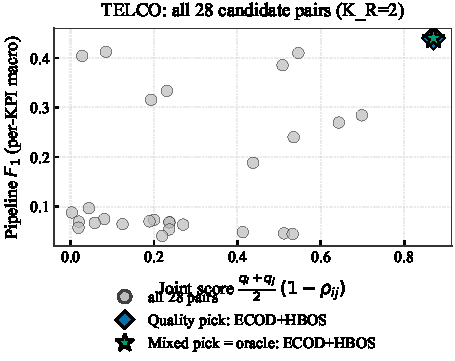
\includegraphics[width=0.95\columnwidth]{figs/fig_jointpair_telco.pdf}
\caption{TELCO: joint pair score versus pipeline $F_1$ for all 28
candidate pairs ($K_R{=}2$). The joint-score maximiser (green star)
coincides with the empirical $F_1$ oracle pair; circled markers are
the runners-up by joint score.}
\label{fig:jointpair}
\end{figure}

\begin{table}[t]
\centering
\caption{TELCO $K_R$ sweep with the self-tuned 10-detector pool and
$\mathcal{S}{=}\text{Mixed}$ selection. The anchor (highest-$q$
member) is LOF throughout; bold marks the peak.}
\label{tab:ksweep}
\scriptsize
\setlength{\tabcolsep}{4pt}
\renewcommand{\arraystretch}{1.0}
\begin{tabular}{clccc}
\toprule
$K_R$ & Selected members (added on each row) & $F_1$ & $P$ & $R$ \\
\midrule
2     & ECOD$+$LOF                                       & 0.384          & 0.567          & 0.315 \\
3     & $+$GMM                                           & 0.462          & 0.595          & 0.426 \\
\textbf{4} & $+$OCSVM                                    & \textbf{0.464} & \textbf{0.605} & 0.425 \\
5     & $+$COPOD                                         & 0.464          & 0.604          & 0.427 \\
6     & $+$IF                                            & 0.456          & 0.592          & 0.431 \\
7     & $+$PCA                                           & 0.456          & 0.595          & 0.431 \\
8     & $+$HBOS                                          & 0.456          & 0.591          & 0.432 \\
9     & $+$KNN                                           & 0.453          & 0.588          & 0.431 \\
10    & $+$AE                                            & 0.455          & 0.592          & \textbf{0.434} \\
\bottomrule
\end{tabular}
\end{table}

\subsection{Per-KPI Breakdown at the Peak Configuration}
\label{sec:res-perkpi}
Table~\ref{tab:perkpi} dissects the $K_R{=}4$ peak run per KPI.
SHAP-$\sigma$ achieves $F_1{>}0.7$ on TS3, TS4, and TS5 (well-behaved
short-burst anomaly types), maintains $F_1{>}0.58$ on six further
KPIs, and fails ($F_1{=}0$) only on the two near-degenerate KPIs
(TS11, TS12) that contain $<25$ ground-truth anomalies each over the
test window. The macro precision of $0.605$ implies that two out of
every three flagged points lie inside a ground-truth anomaly
segment.

\begin{table}[t]
\centering
\caption{Per-KPI breakdown at the peak $K_R{=}4$ configuration
(ECOD$+$LOF$+$GMM$+$OCSVM, anchor LOF). \emph{$\#$true}: number of
labelled anomaly timestamps; \emph{$\#$pred}: number of pipeline
flags; TP/FP/FN are confusion-matrix counts.}
\label{tab:perkpi}
\scriptsize
\setlength{\tabcolsep}{3pt}
\renewcommand{\arraystretch}{1.0}
\begin{tabular}{lrrrrrccc}
\toprule
KPI  & $\#$true & $\#$pred & TP  & FP  & FN  & $F_1$ & $P$ & $R$ \\
\midrule
TS1  & 412      & 144      & 104 & 40  & 308 & 0.374 & 0.722 & 0.252 \\
TS2  & 501      & 147      & 118 & 29  & 383 & 0.364 & 0.803 & 0.236 \\
TS3  & 138      & 165      & 121 & 44  & 17  & \textbf{0.799} & 0.733 & \textbf{0.877} \\
TS4  & 179      & 163      & 127 & 36  & 52  & 0.743 & 0.779 & 0.709 \\
TS5  & 106      & 125      & 92  & 33  & 14  & 0.797 & 0.736 & 0.868 \\
TS6  & 107      & 140      & 78  & 62  & 29  & 0.632 & 0.557 & 0.729 \\
TS7  & 269      & 189      & 133 & 56  & 136 & 0.581 & 0.704 & 0.494 \\
TS8  & 267      & 175      & 135 & 40  & 132 & 0.611 & 0.771 & 0.506 \\
TS9  & 564      & 148      & 115 & 33  & 449 & 0.323 & 0.777 & 0.204 \\
TS10 & 501      & 170      & 115 & 55  & 386 & 0.343 & 0.676 & 0.230 \\
TS11 & 21       & 61       & 0   & 61  & 21  & 0.000 & 0.000 & 0.000 \\
TS12 & 15       & 102      & 0   & 102 & 15  & 0.000 & 0.000 & 0.000 \\
\midrule
macro & 3{,}080  & 1{,}729  &     &     &     & \textbf{0.464} & \textbf{0.605} & 0.425 \\
\bottomrule
\end{tabular}
\end{table}

\subsection{Comparison to Deep Baselines}
\label{sec:res-deep}
Table~\ref{tab:summary} compares SHAP-$\sigma$ at $K_R{=}4$ against
the released deep baselines on the per-KPI macro $F_1$ used
by~\cite{Malacarne2026}. SHAP-$\sigma$ is $3.5\times$ above DC-VAE
($F_1{=}0.134$~\cite{gonzalez2023one}) and $2.9\times$ above
C-MTAD-GAT ($F_1{=}0.160$~\cite{Malacarne2026}) under the same
evaluation window.

\begin{table}[t]
\centering
\caption{TELCO headline: per-KPI macro metrics for the best
self-tuned singleton, the canonical SHAP-$\sigma$ pipeline at the
peak Rashomon size, and the two released deep baselines. Bold $=$
best per column.}
\label{tab:summary}
\footnotesize
\setlength{\tabcolsep}{4pt}
\renewcommand{\arraystretch}{1.05}
\begin{tabular}{lccc}
\toprule
Method & $F_1$ & $P$ & $R$ \\
\midrule
DC-VAE~\cite{gonzalez2023one}            & 0.134           & ---             & --- \\
C-MTAD-GAT~\cite{Malacarne2026}          & 0.160           & ---             & --- \\
\addlinespace[1pt]
self-tuned LOF (best singleton)           & 0.419           & 0.460           & \textbf{0.452} \\
\textbf{SHAP-$\sigma$ ($K_R{=}4$, Mixed)} & \textbf{0.464}  & \textbf{0.605}  & 0.425 \\
\bottomrule
\end{tabular}
\end{table}

\section{Conclusions}
\label{sec:conclusion}

We presented SHAP-$\sigma$, a label-free pipeline for multivariate
cellular network anomaly detection that promotes the cross-detector
standard deviation of SHAP attributions from a post-hoc explanation
into a first-class attribution-evidence signal. The methodological
contributions are: (i) label-free self-tuning of a $K{=}10$
unsupervised detector pool (including an AutoEncoder and OCSVM
alongside the eight standard PyOD detectors); (ii) a closed-form
Rashomon pair score
$\tfrac{q_i+q_j}{2}(1-\rho_{ij})$ combining a Mass--Volume proxy with
a cardinality veto; and (iii) a per-KPI $\sigma$ gate that filters
anchor flags by the cross-detector spread of TreeSHAP attributions.
On the TELCO cellular benchmark a $K_R$ sweep peaks at $K_R{=}4$
with the self-tuned quartet $\{$ECOD, LOF, GMM, OCSVM$\}$, reaching
per-KPI macro $F_1{=}0.464$ (precision $0.605$, recall $0.425$),
$+0.045$ over the best self-tuned singleton. The pipeline exceeds the
released deep baselines DC-VAE and
C-MTAD-GAT~\cite{Malacarne2026,gonzalez2023one} by $2.9$--$3.5\times$
on the same evaluation window, while remaining transparent and
reproducible per-KPI.

\paragraph{Limitations and future work.}
Eq.~\eqref{eq:final} is recall-monotone with respect to the anchor
singleton; the disjunctive feature-wise gate is most informative on
per-feature labels (as in TELCO) and degenerates under
OR-aggregation for point-level multivariate evaluation, which we
defer to a journal extension on extended cellular benchmarks. We
also plan to learn $(K_R,\mathcal{S})$ label-free from synthetic
anomaly injection~\cite{Goswami2023,Zhao2021}, to compare against
recent deep label-free baselines such as
MTGFlow~\cite{zhou2023labelfree}, and to extend $\sigma$-SHAP to
cross-window variance for streaming deployment.

\balance
\bibliographystyle{IEEEtran}
\bibliography{references}

\end{document}
